\documentclass[twoside]{article}
\usepackage[a4paper]{geometry}
\geometry{verbose,tmargin=2.5cm,bmargin=2cm,lmargin=2cm,rmargin=2cm}
\usepackage{fancyhdr}
\pagestyle{fancy}

% nastavení pisma a~češtiny
\usepackage{lmodern}
\usepackage[T1]{fontenc}
\usepackage[utf8]{inputenc}
\usepackage[czech]{babel}

% odkazy
\usepackage{url}

\usepackage{float}
% vícesloupcové tabulky
\usepackage{multirow}
\usepackage{amssymb}
\usepackage{gensymb}
\usepackage{bbold}
\usepackage{amsmath}
\usepackage{mathtools}
\usepackage{commath}

% vnořené popisky obrázků
\usepackage{subcaption}

% automatická konverze EPS 
\usepackage{graphicx} 
\usepackage{epstopdf}
\epstopdfsetup{update}

\graphicspath{{./images}}

% odkazy a~záložky
\usepackage[unicode=true, bookmarks=true,bookmarksnumbered=true,
bookmarksopen=false, breaklinks=false,pdfborder={0 0 0},
pdfpagemode=UseNone,backref=false,colorlinks=true] {hyperref}

% Poznámky při překladu
\usepackage{xkeyval}	% Inline todonotes
\usepackage[textsize = footnotesize]{todonotes}
\presetkeys{todonotes}{inline}{}

%https://tex.stackexchange.com/questions/2783/bold-calligraphic-typeface
\DeclareMathAlphabet\mathbfcal{OMS}{cmsy}{b}{n}

% Zacni sekci slovem ukol
\renewcommand{\thesection}{Úkol \arabic{section}}
% enumerate zacina s pismenem
\renewcommand{\theenumi}{\alph{enumi}}

% smaz aktualni page layout
\fancyhf{}
% zahlavi
\usepackage{titling}
\fancyhf[HC]{\thetitle}
\fancyhf[HLE,HRO]{\theauthor}
\fancyhf[HRE,HLO]{\today}
 %zapati
\fancyhf[FLE,FRO]{\thepage}

% údaje o autorovi
\title{Protokol - pokročilé použítí osciloskopu}
\author{Vojtěch Michal}
\date{\today}

\begin{document}

\maketitle

\section{Harmonické signály}

\subsection{Měření charakteristik}
\begin{figure}[htbp]
	\centering
	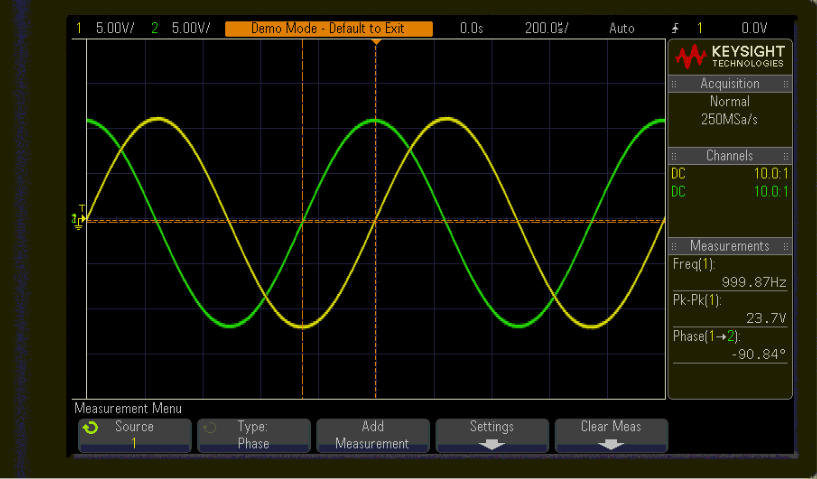
\includegraphics[width=.6\linewidth]{sinus_frek_pp_automatika.png}
\caption{Charakteristiky měřené automaticky}
\end{figure}

\begin{figure}[htbp]
	\centering
	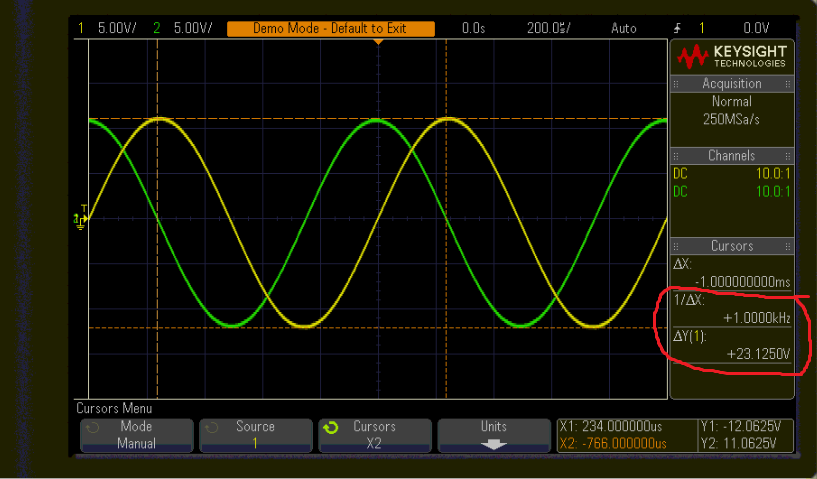
\includegraphics[width=.6\linewidth]{sinus_frek_pp_kurzor.png              }
	\caption{Charakteristiky měřené kurzorem}
\end{figure}

Automatika je schopna měřit až tehdy, když vidí na obrazovce celou periodu,
zatímco člověk může "tipnout" hodnotu rovnou. Ovšem protože jsou k dispozici jenom dva kurzory na každou osu
(a víc by ani nebylo ovladatělných pro nepřehlednost), nelze třeba jednoduše naráz kurzorem změřit fázi i frekvenci.
Kdyby nebyly signály ideální, ale třeba by trošku fluktuovalo Vpp, je automatické měření k nezaplacení - má cca tak
nekonečněkrát vyšší obnovovací frekvenci než člověk vůbec zpozoruje, že kurzory již nejsou na správných místech.

%\begin{figure}[htbp]
%    \centering % <-- added
%\begin{subfigure}{0.45\textwidth}
%  \includegraphics[width=\linewidth]{graph33_vstup1.eps}
%  \caption{Simulace pro vstup $u(t) = 1$}
%\end{subfigure}\hfil % <-- added
%\begin{subfigure}{0.45\textwidth}
%	\includegraphics[width=\linewidth]{graph33_vstup2.eps}
%	\caption{Simulace pro vstup $u(t) = 2.001$}
%\end{subfigure}
%\caption{Simulace odezev nelineárního a linearizovaného systému na různé vstupy}
%\label{fig:linearizace}
%\end{figure}

\subsection{XY zobrazení}
Užitečné pro sledování fázového rozdílu dvou signálů na stejné frekvenci.
Pakliže se frekvence liší, začne se signál pohybovat, jak se mění okamžitý fázový posun.
\begin{figure}[htbp]
	
	\begin{subfigure}{0.3\textwidth}
		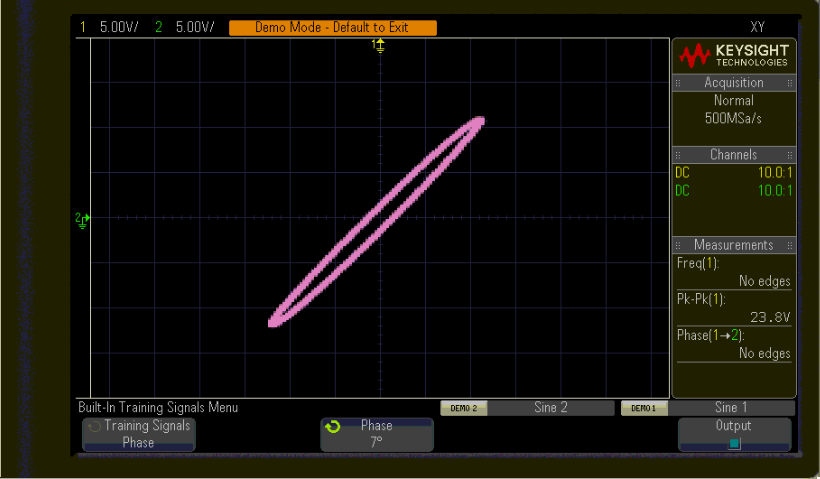
\includegraphics[width=\linewidth]{xy_7deg.png}
	\end{subfigure}
	\begin{subfigure}{0.3\textwidth}
		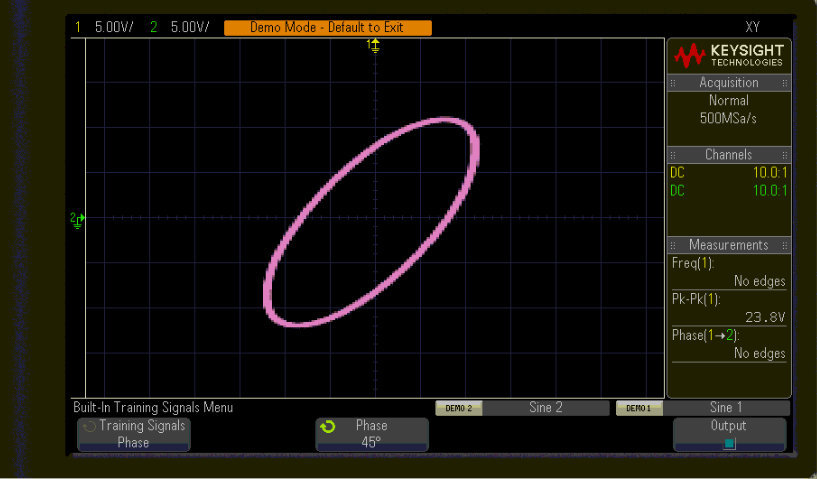
\includegraphics[width=\linewidth]{xy_45deg.png}
	\end{subfigure}
	\begin{subfigure}{0.3\textwidth}
		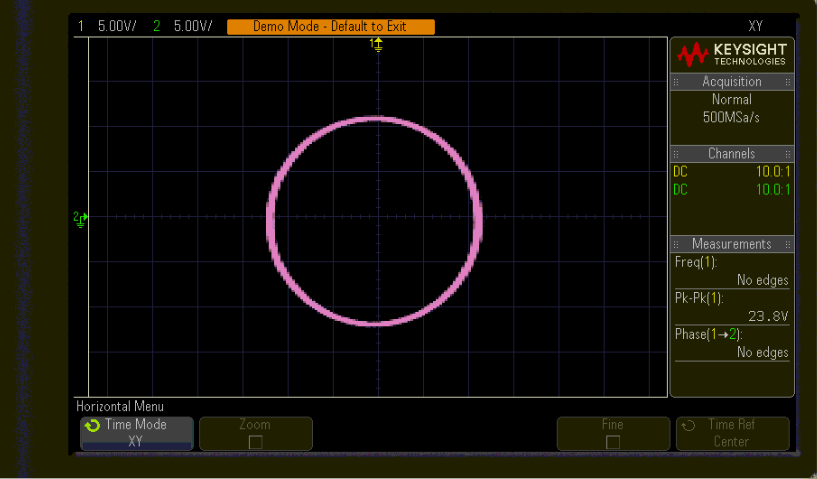
\includegraphics[width=\linewidth]{xy_90deg.png}
	\end{subfigure}
	\caption{XY zobrazení fázově posunutých signálů. Zleva doprava fázový rozdíl 7°, 45° a 90°}
\end{figure}

\subsection{Matematika}
\begin{figure}[htbp]
	\centering
	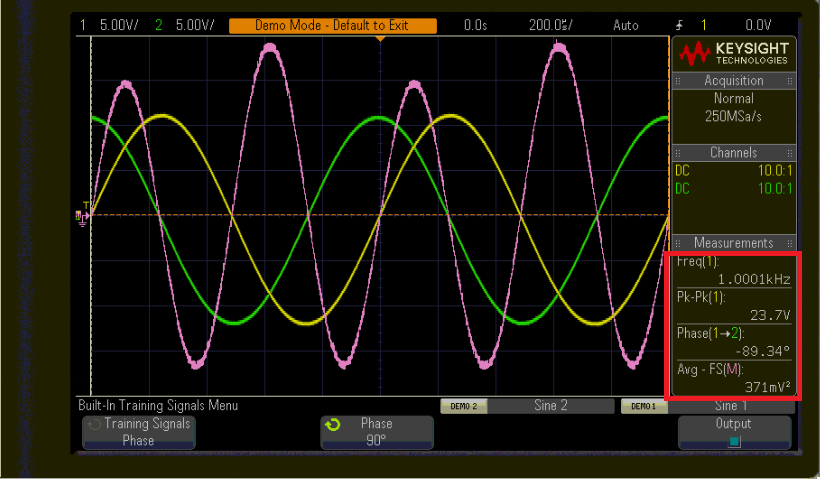
\includegraphics[width=.6\linewidth]{sinus_matematika_stredni_hodnota.png  }
	\label{fig:vykon}
\end{figure}
Pakliže by harmonické signály představovaly proud a napětí, jejich součin bude odpovídat okamžitému výkonu,
což bude harmonický signál na dvojnásobné frekvenci.
Integrací přes nějaký časový úsek (ideálně periodu)a rozkladem na složky vzniká činný a jalový výkon.
Činný výkon bude nulový na prvcích bez ohmického odporu, tedy L či C. Konkrétně na \ref{fig:vykon},
pakliže by kanál 1 (žlutý) byl napětím a kanál 2 (zelený) byl proudem, poté máme průběh
veličin na kapacitoru a činný výkon je nulový (fázový rozdíl I a U je $\frac{\pi}{2}$). 


\section{Trigger}

Když je na vstupu signál a je splněna trigger condition (například signál projde nastavenou úrovní),
jsou módy identické. Když trigger condition splněna není, potom normal mode jen sampluje a čeká
(symbol otazníku u Trig v horním pravém rohu), zatímco autotrigger čas od času pustí vzorkování a vykreslí
průběh. Protože vzorkování není synchronizováno, jsou průběhy kresleny náhodně a na displeji vzniká
barevná mlha. Alespoň je ale vidět, že je připojen nějaký signál.

\begin{figure}[htbp]
	\centering
	\begin{subfigure}{0.45\textwidth}
		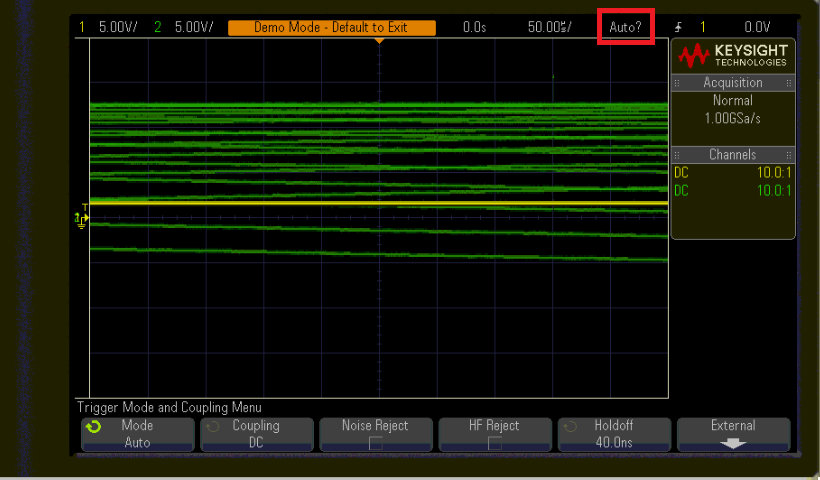
\includegraphics[width=\linewidth]{trigger_auto.png                      }
		\caption{Auto trigger (bez triggeru)}
	\end{subfigure}
	\begin{subfigure}{0.45\textwidth}
		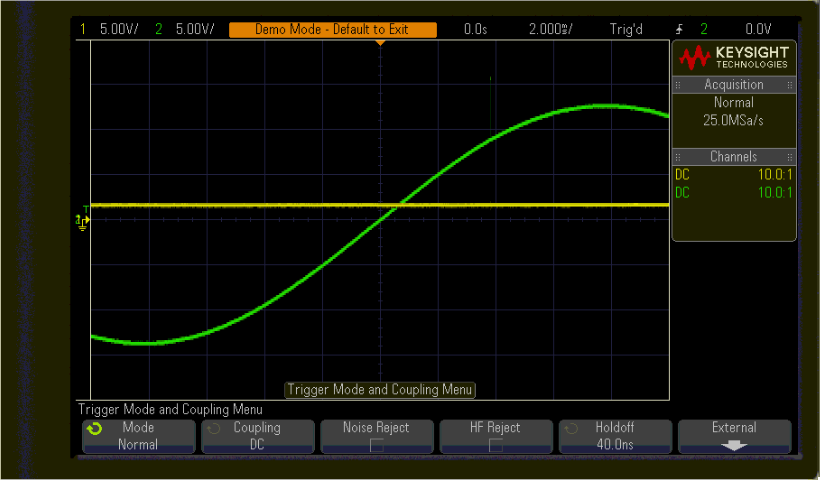
\includegraphics[width=\linewidth]{trigger_normal.png                    }
		\caption{Normal mode (trigger condition splněna)}
	\end{subfigure}
\end{figure}

Režim auto je tak vhodný pro získání všeobecného přehledu o signálu (jestli se vejde na vertikální)
stupnici, jestli je jen pulsní či periodický (barevná mlha různých průběhů je tak nějak rozumně rozložena a dílčí průběhy
vypadají podle očekávání) atd.


	
		
		\begin{thebibliography}{9}
			
			
			\bibitem{zadani}
			, \url{https://moodle.fel.cvut.cz/pluginfile.php/296878/mod_resource/content/1/advanced_remote_scope_v2.pdf}
			
			\bibitem{motivace}
			Motivační hudba, \emph{Kirby dream land theme song} \url{https://www.youtube.com/watch?v=3CS93CdMv_E}
			
		\end{thebibliography}
		
		\end{document}
		
		